\section*{Introduction}
Le développement de modules de noyau sous Linux offre une puissante méthode pour étendre ou personnaliser le comportement du noyau. Un module de noyau est un programme qui peut être dynamiquement chargé et déchargé dans le noyau du système d'exploitation sans nécessiter de redémarrage. Ces modules fournissent une manière flexible d'ajouter des fonctionnalités au noyau sans avoir à recompiler l'ensemble du noyau ou à modifier le code source du noyau directement.
\section{Installation des package nécessaires}
\textbf{sudo apt-get install build-essential linux-headers-(uname -r)}
\section{Création du répertoire du module}
\textbf{mkdir kernel\_modules}
\\\textbf{cd kernel\_modules}
\section{Création du fichier source du module}
\begin{figure}[h]
    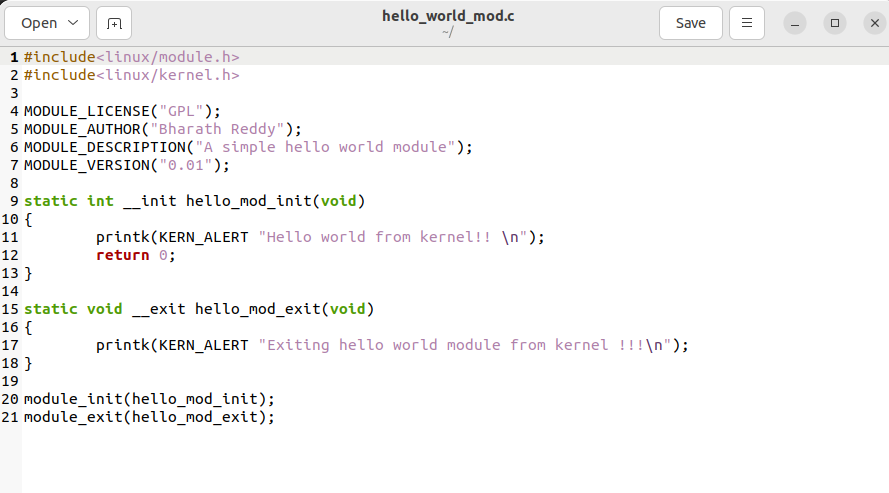
\includegraphics[width=0.8\textwidth]{images/47.png}   
\end{figure}

Ce code crée un module de noyau simple qui, lorsqu'il est chargé, écrit "Hello world from kernel!!" dans les logs du noyau, et lorsqu'il est déchargé, écrit "Exiting hello world module from kernel !!!"

\section{Création du fichier Makefile}

Le fichier Makefile dans le contexte du développement de modules de noyau sous Linux est un script utilisé par l'utilitaire make pour automatiser le processus de compilation. Son rôle est de spécifier comment les fichiers source doivent être compilés et liés pour créer le module de noyau.
\begin{figure}[h]
    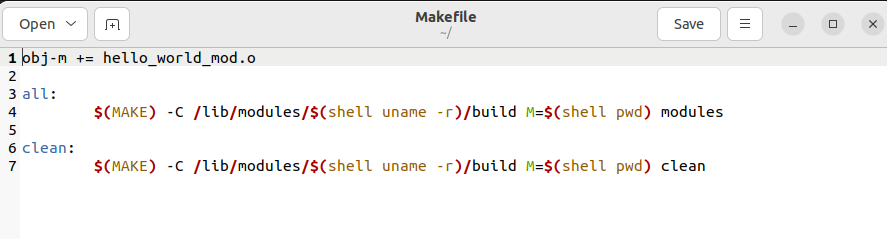
\includegraphics[width=0.8\textwidth]{images/48.png}   
\end{figure}
\\Ce fichier est conçu pour être utilisé avec le système de construction du noyau Linux. La cible all compile le module, tandis que la cible clean supprime les fichiers temporaires générés lors de la compilation. Ces commandes simplifient le processus de compilation et de nettoyage des modules du noyau.
\section{Compilation du module}
\textbf{make all}
\begin{figure}[h]
    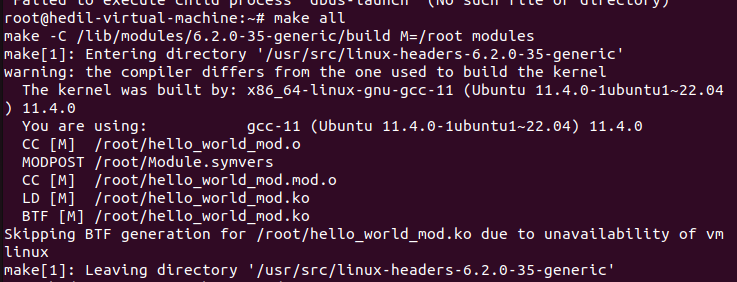
\includegraphics[width=0.8\textwidth]{images/49.png}   
\end{figure}

\section{Chargerment du module}
\begin{figure}[h]
    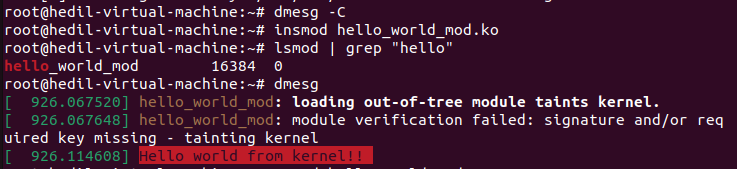
\includegraphics[width=0.8\textwidth]{images/50.png}   
\end{figure}
\newpage
\textbf{1- Réinitialisation du tampon des messages du noyau}
\\dmesg -c

\\\textbf{2- Chargerment du module}
\\sudo insmod hello\_world\_mod.ko

\textbf{3- Vérifier le chargement du module}
\\lsmod | grep "hello"

\\\textbf{4- Vérifier les journaux système (dmesg) }
\\dmesg

\section{Déchargerment du module}

\begin{figure}[h]
    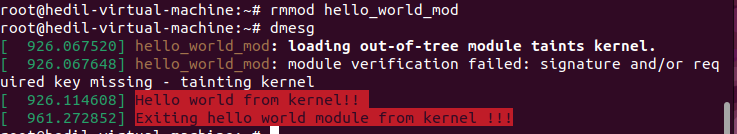
\includegraphics[width=0.8\textwidth]{images/51.png}   
\end{figure}


\\\textbf{1- Déhargerment du module}
\\sudo rmod hello\_world\_mod.ko


\\\textbf{2- Vérifier les journaux système (dmesg) }
\\dmesg

\section*{Conclusion}
Cette tâche a démontré les concepts fondamentaux du développement de modules de noyau, offrant un aperçu de la manière dont ces modules peuvent être utilisés pour étendre la fonctionnalité du noyau Linux de manière dynamique et flexible. Elle constitue une base solide pour des projets plus avancés impliquant des modules de noyau personnalisés.